\chapter{Testing isotropy and Gaussianity in the \textit{Planck} CMB estimates (preliminary results)}
\label{chapter-vsk}

\section{Introduction} 

The cosmological principle -- the assumption that the universe at sufficiently large scales is homogeneous and isotropic -- is one of the cornerstones of the standard model of cosmology (see, e.g., \cite{Robertson:1935zz,Walker1937,Hogg:2004vw}). Any significant indication of its violation would mean a serious caveat in our cosmological paradigm. Therefore, to examine the validity of these assumptions is crucial. 

Recently, the \textit{Planck} collaboration has measured the anisotropies in the CMB with a much better precision than the \textit{Wilkinson Microwave Anisotropy Probe} (hereafter, \textit{WMAP}) (see, e.g., \cite{Spergel:2003cb}). According to the inflationary paradigm, at very early times the universe was filled with a hypothetical scalar field, the inflaton, whose fluctuations produced curvature perturbations distributed as a homogeneous and isotropic Gaussian random field. Cosmological perturbation theory establishes a relation between those primordial fluctuations and the CMB anisotropies, hence offering a unique probe to test models of the early universe. This relation implies that, in the framework of the cosmological principle, the CMB anisotropies are  statistically isotropic and Gaussian. Thence, testing the statistical properties of the CMB anisotropies allows us to examine  basic assumptions of the standard model of cosmology. In this chapter we will apply a statistical method different to those used by the \textit{Planck} team in \cite{Ade:2013nlj} to look for possible deviations of Gaussianity and isotropy in the \textit{Planck} data.

The \textit{WMAP} team \cite{Spergel:2003cb} and other groups found some unexpected features -- anomalous properties in the CMB anisotropies which are statistically inconsistent with a best-fit $\Lambda$CDM model -- especially on large angular scales ($\ell < 600$). The list of anomalies includes lack of power on large angular scales \cite{Copi:2006tu}, alignment of low-order multipoles \cite{Tegmark:2003ve,Schwarz:2004gk,Bielewicz:2005zu,Land:2005ad}, north-south asymmetry in both power spectra \cite{Eriksen:2003db,Hansen:2008ym} and several measures of non-Gaussianity \cite{Eriksen:2004df,Eriksen:2004iu,Rath:2007ti,Rossmanith:2009cy}, the cold spot \cite{Vielva:2003et,Cruz:2004ce}, and parity asymmetry in the power spectrum \cite{Kim:2010gf}. Not long ago, the \textit{Planck} team has confirmed the observation of those large scale anomalies. Bearing in mind that both \textit{Planck} and \textit{WMAP} are cosmic variance limited, the presence of those unexpected features in the \textit{WMAP} and \textit{Planck} data could be, in principle, due to unaccounted systematic errors, non-subtracted foreground contamination, or more interestingly, it could have a cosmological origin. On the one hand, the fact that two independent experiments have observed the same features reduces drastically the possibility that systematics errors be the source of these anomalies \cite{Larson:2014roa}. On the other hand, unresolved foreground and the more appealing cosmological origin need to be studied further. 

In \cite{Ade:2013nlj} the \textit{Plank} team tested the Gaussianity and isotropy of  the CMB anisotropies and determined the statistical significance of their findings with a set of Gaussian, isotropic simulations of the CMB sky, namely, the ``Full Focal Plane'' (FFP6) simulations. They used several statistical methods including the study of one-dimensional moments, N-point correlation functions, Minkowski functionals, wavelet, bispectrum and phase correlations. Several of those statistical methods (e.g., N-point correlation functions, the Minkowski functionals, and the bispectrum) show consistency with Gaussianity and isotropy regardless of the mask, the component separation and the resolution of the CMB maps (i.e., $N_{side}$). Nevertheless, there is inconsistency with the FFP6 simulations when other methods are utilised. In their one-dimensional moments analysis they found that the variance is anomalously low at all considered resolutions ($N_{side}=2048,\, 512,\, 64,\, 32,\, 16$) and that the skewness (kurtosis) is anomalously low (high) at low resolutions ($N_{side}=64,\,32,\,16$). When using the wavelet statistics they also found inconsistencies. In particular, they report skewness (kurtosis) at small (intermediate) scales significantly lower (greater) than in the simulations. Finally, the most important discrepancy between data and simulations appears when analysing the data with the method of surrogates. The \textit{Planck} team found presence of pronounced anisotropy and also correlations between the low-$\ell$ Fourier phases in the analysed CMB maps, findings which turn out to be robust regardless of reference frame and component separation method. Similar results were obtained previously in \textit{WMAP} data \cite{Rossmanith:2009cy}. 

It is of great importance for the standard model of cosmology to clarify these discrepancies between the isotropic, Gaussian simulations and the \textit{Planck} data. In this chapter we use the VSK method to test isotropy and Gaussianity with a set of Gaussian, isotropic simulations of the CMB sky. The VSK method consists of a set of statistical estimators which measure variance, skewness, and kurtosis in patches of the sky. The VSK method is similar to the wavelet statistics employed by the \textit{Planck} collaboration but, since our analysis works in real space, it localizes possible non-subtracted foregrounds and may provide the angular scale of possible deviations of Gaussianity and isotropy in the CMB anisotropies. Recently, a similar approach was used in \cite{Bernui:2014oda} and in \cite{Bernui:2014gla} to study the north-south asymmetry phenomenon and non-Gaussianity in CMB anisotropies, respectively. However, the authors used overlapping patches of the sky when defining their estimators, possibly introducing spurious correlations in their estimations. Moreover, they did not use CMB maps in the full \textit{Planck} resolution ($N_{side}=2048$); even though this reduces the noise in the data (dominant at small scales), it also increases the error in the estimations. Using maps with lower resolution could make the error bars larger.

In the present chapter, we start out giving a brief description of the data (Section \ref{s:data}) and then present the VSK method for non-overlapping patches of the sky (Section \ref{s:method}). The VSK method is subsequently applied to both \textit{Planck} data and Gaussian, isotropic simulations of the CMB sky and our results are discussed in Section \ref{s:results}. We conclude in Section \ref{s:summary}.

\section{Data}
\label{s:data}

Here we analyse of part of the 2013 \textit{Planck} data release corresponding to the nominal period of the \textit{Planck} mission. We utilise some of the available masks, the two available inpainted CMB maps, and the nearly full-sky foreground cleaned CMB maps resulting from four  component separation algorithms applied by the \textit{Planck} team \cite{Ade:2013crn}, viz., \texttt{Commander-Ruler, NILC, SEVEM} and \texttt{SMICA}. The maps and masks were provided in \textsc{HEALPix}\footnote{http://healpix.sourceforge.net} format, with a pixel size defined by the $N_{side}$ parameter. 

Throughout the paper we use the standardized common mask U73 (sky coverage $f_{sky} = 73$ per cent). However, when studying the mask dependence of our analysis we use the confidence mask VALMASK ($f_{sky} = 89$ per cent) and the mask of the inpainted regions INP$\_$MASK ($f_{sky} = 97$ per cent) of the \texttt{SMICA} CMB estimate. Where appropriate, we have changed the resolution of the mask and maps, originally having $N_{side}=2048$. In particular, we have degraded the data to have $N_{side}=1024,\, 512$, and $256$. When degrading the mask we have followed a conservative approach: after degrading the mask to the final resolution using the \textsc{ud$\_$grade HEALPix} routine, any pixel having a value lower than $0.9$ has been set to zero. 

Finally, in order to assess the significance of any anisotropic or non-Gaussian signal in the data, we resort to a set of $2000$ simulated Gaussian, isotropic CMB maps. The Monte Carlo simulations were generated using the \textsc{synfast HEALPix} routine based on the \textit{Planck} best-fit power spectrum and having an effective Gaussian beam $\texttt{FWHM}=5$ arcmin.

\section{VSK Method}
\label{s:method}

The method, which in the scope of this study will be referred to as VSK method, was first introduced and applied to \textit{WMAP} data in \cite{Bernui:2008ei}  (see also \cite{Bernui:2009wq,Bernui:2011yj}). However, as originally proposed, the method uses overlapping patches in the sky that, as mentioned earlier, might introduce spurious correlations in the data. The VSK method was modified to employ non-overlapping patches of the sky and applied to \textit{WMAP} data in \cite{Cardona:2013pqa} and simulations in \cite{Cardona:2013fxa}. Given a full-sky CMB map in \textsc{HEALPix} format with parameter $N_{side}$, the construction of the estimators in the VSK method proceeds as follows. 

\begin{enumerate}
\item We remove both monopole and dipole with the \textsc{remove$\_$dipole} \\ \textsc{HEALPix} routine 
\item We superimpose on the original CMB map a \textsc{HEALPix} grid with much lower resolution $N'_{side}$ than that of the CMB map (e.g., $N'_{side} = 2,4,8,\dots$). Thus, we have a set of $12 \times N^{'2}_{side}$ non-overlapping patches in the sky, each patch having equal number $N_p$ of pixels belonging to the initial CMB map\footnote{For a full-sky CMB map with parameter $N_{side}$ the number of pixels is given by $12 \times N^2_{side}$. Then, the number of pixels per patch is given by $\left(N_{side}/N'_{side}\right)^2$.}. %Hereafter, we will call each one of those non-overlapping patches cells.
\item For each patch we compute sample variance,
\begin{equation}
\label{eq:1}
V_j = \frac{1}{N_p -1} \sum_{i=1}^{N_p} (T_i - \bar{T})^2 = \frac{N_p}{N_p -1} \sigma_j^2 ,
\end{equation}
sample skewness,
\begin{equation}
\label{eq:2}
S_j = \frac{1}{N_p \sigma_j^3} \sum_{i=1}^{N_p} (T_i - \bar{T})^3 ,
\end{equation}
and sample kurtosis,
\begin{equation}
\label{eq:3}
K_j = \frac{1}{N_p \sigma_j^4} \sum_{i=1}^{N_p} (T_i - \bar{T})^4 - 3 ,
\end{equation}
where $j$ numbers the non-overlapping patches, $T_i$ is the temperature at the $i^{th}$ pixel in the $j^{th}$ patch, $\bar{T}$ is the CMB mean temperature in the $j^{th}$ patch, and $\sigma_j$ denotes the standard deviation of the CMB data in the $j^{th}$ patch. We compute sample variance, sample skewness, and sample kurtosis including only unmasked pixels; any patch for which more than $20$ per cent of the area is masked is set to zero.
\item The result of computing $V_j$, $S_j$, and $K_j$ for all the patches is three different maps, namely, one map of sample variance, one map of sample skewness and one map of sample kurtosis. 
\item We repeat the four items above for the set of $2000$ Gaussian, isotropic simulations CMB maps and compute zero mean sample variance maps, zero mean sample skewness maps, and zero mean sample kurtosis maps. Henceforward, we will refer to a given zero mean map as V-map, S-map and K-map, respectively.
\item Since the V-map, S-map, and the K-map are signals on the sphere, they can be written in terms of a spectral representation. For instance, for the V-map we have 
\begin{equation}
\label{eq:4}
V(\mathbf{x}) = \sum^{\infty}_{\ell=0} \sum^{\ell}_{m=-\ell} v_{\ell m} Y_{\ell m} (\mathbf{x})
\end{equation}

\noindent where $\mathbf{x}$ is a unit direction vector, $Y_{\ell m}$ the spherical harmonics and 

\begin{equation}
v_{\ell m} = \int d\mathbf{x} V(\mathbf{x}) Y^*_{\ell m}(\mathbf{x}),
\end{equation}

\noindent $m=0,\pm1,\dots,\pm \ell$, $\ell=0,1,2,\dots$. Similar expressions are satisfied by both S-map and K-map. 

\item Finally, we perform the harmonic analysis of the V-map, S-map, and K-map with the help of the \textsc{anafast HEALPix} routine with maximum spherical harmonic order given by $\ell_{max}=3\times N'_{side}-1$. Taking as an example the $V(\mathbf{x})$ signal again, we have 
\begin{equation}
\label{eq:5}
V_\ell = \frac{1}{2 \ell +1} \sum_{m} |v_{\ell m}|^2 ,
\end{equation}
where $V_{\ell}$ is the angular power spectrum of the V-map. Similar expressions  $S_\ell$ and $K_\ell$ apply for S-map and K-map, respectively.
\end{enumerate}

Throughout this chapter we quantify the degree of agreement between the Gaussian, isotropic simulations and the observations by a simple $\chi^2$ test which has been performed separately for the V, S, and K estimators. For instance, for the V estimator we define $\chi^2_{V}$ as 

\begin{equation}
\chi^2_{V} = \sum_{\ell \ell'} \left( V_\ell - \left\langle V_\ell \right\rangle_G \right) C^{-1}_{\ell \ell'} \left( V_{\ell'} - \left\langle V_{\ell'} \right\rangle_G\right),
\label{eq:6}
\end{equation}

with analogous expressions for S and K estimators. In equation (\ref{eq:6}) $V_\ell$ is the angular power spectrum of a V-map computed out of a given full-sky CMB map, $\left\langle V_\ell \right\rangle_G$ the corresponding average from the first $1000$ Gaussian, isotropic simulations, and 

\begin{equation}
C_{\ell \ell'} = \left\langle \left( V_\ell - \left\langle V_\ell \right\rangle_G \right) \left( V_{\ell'} - \left\langle V_{\ell'} \right\rangle_G \right)\right\rangle_G
\end{equation}

the covariance matrix from the remaining $1000$  Gaussian, isotropic simulations.

\section{Results}
\label{s:results}

We now apply the VSK method to the \textit{Planck} data. We start by examining how the method works when using full-sky ($f_{sky}=100$ per cent) CMB maps. In particular, we use the two inpainted CMB estimates released by the \textit{Planck} collaboration, namely, the $N_{side}=2048$ inpainted \texttt{SMICA} and \texttt{NILC}. 

Figures \ref{Fig:0a}--\ref{Fig:0c} show V-map, S-map, and K-map for the inpainted \texttt{SMICA}. In Figures \ref{Fig:1}--\ref{Fig:1b} we plot angular power spectra for the V-map, S-map, and the K-map computed for both inpainted \texttt{SMICA} and \texttt{NILC} CMB estimates, as well as for $1000$ Gaussian, isotropic simulations using $N'_{side} = 2$. The mean angular power spectra for the simulations do not exhibit any strong scale dependence. The angular power spectrum of the variance maps, $V_{\ell}$, for the two considered CMB estimates show no departure from the null hypothesis. %In particular, inpainted \texttt{SMICA} has both a dipole and a quadrupole outside the $95$ per cent confidence region. 
The VSK method does not bring about any dipolar structure in the inpainted CMB estimates; this so-called north-south asymmetry, was found in \textit{WMAP} and \textit{Planck} data \cite{Eriksen:2003db,Hansen:2008ym,Ade:2013nlj,Akrami:2014eta}. Using different values of the parameter $N'_{side}$, we are verifying the robustness of this result for the inpainted CMB maps. The angular power spectra of the corresponding S-maps, $S_{\ell}$, is consistent with the null hypothesis. 
%Although at multipoles $\ell \geq 10$ the inpainted \texttt{NILC} shows  a little tension with regard to the simulations, we could verify that this mismatch vanishes when $N'_{side}$ increases. 
The most remarkable difference between the two CMB estimates is brought out when looking at the corresponding $K_{\ell}$. The inpainting technique applied to the \texttt{NILC} CMB estimate seems to induce kurtosis at all considered scales. We checked that this contribution vanishes when the inpainted region is masked (see Figure \ref{Fig:4b}). %The same applies for the multipole $\ell=5$ in the inpainted \texttt{SMICA}. 
In Figures \ref{Fig:2}--\ref{Fig:2b} we show the $\chi^2$ analyses for the spectra in Figures \ref{Fig:1}--\ref{Fig:1b}. Note that due to the discrepancy in the inpainted \texttt{NILC}, we do not show its $\chi^2$ value for $K_{\ell}$. In Table \ref{table:1} we show the lower-tail probability computed out of N-pdf $\chi^2$ for different values of the parameter $N'_{side}$. The V, S, and K estimators give consistent results for the two CMB estimates and we are studying whether or not the results depend on the $N'_{side}$ parameter. %The probabilities are high for all the $N'_{side}$ considered. The probabilities for the S estimator vary consistently with $N'_{side}$. However, for $N'_{side}=4$ the probability is high in the inpainted \texttt{NILC}. The probabilities for the K estimator increase with $N'_{side}$ for inpainted \texttt{SMICA} and remain constant for inpainted \texttt{NILC} because of the discrepancy shown we discussed previously.
The only discrepancy appears for the K-map inpainted \texttt{NILC} that is fully inconsistent with the Gaussian, isotropic simulations. 

\begin{figure}
\centering
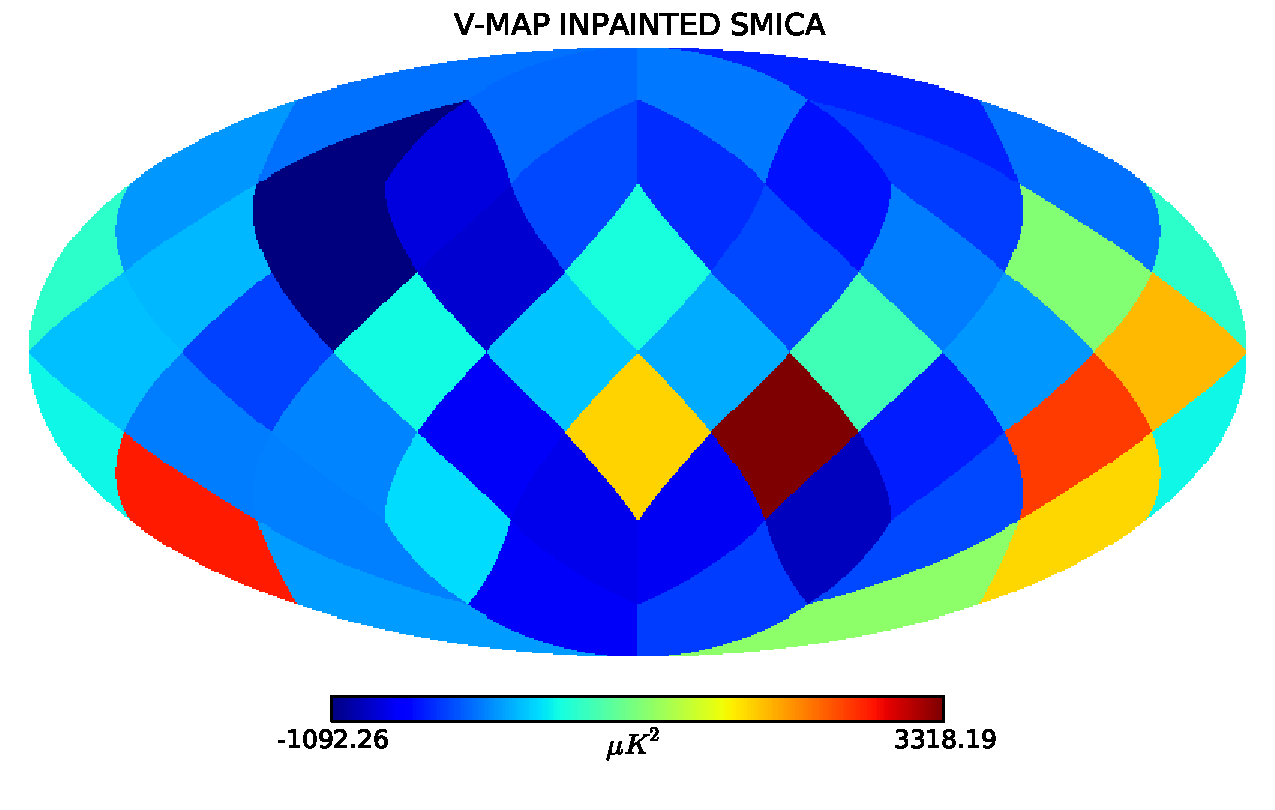
\includegraphics[width=\textwidth]{figures/chapter-vsk/vmap-inpainted-smica.pdf}
\caption{$N'_{side = 2}$ V-map for the $N_{side} = 2048$ inpainted SMICA CMB estimate.}
\label{Fig:0a}
\end{figure}

\begin{figure}
\centering
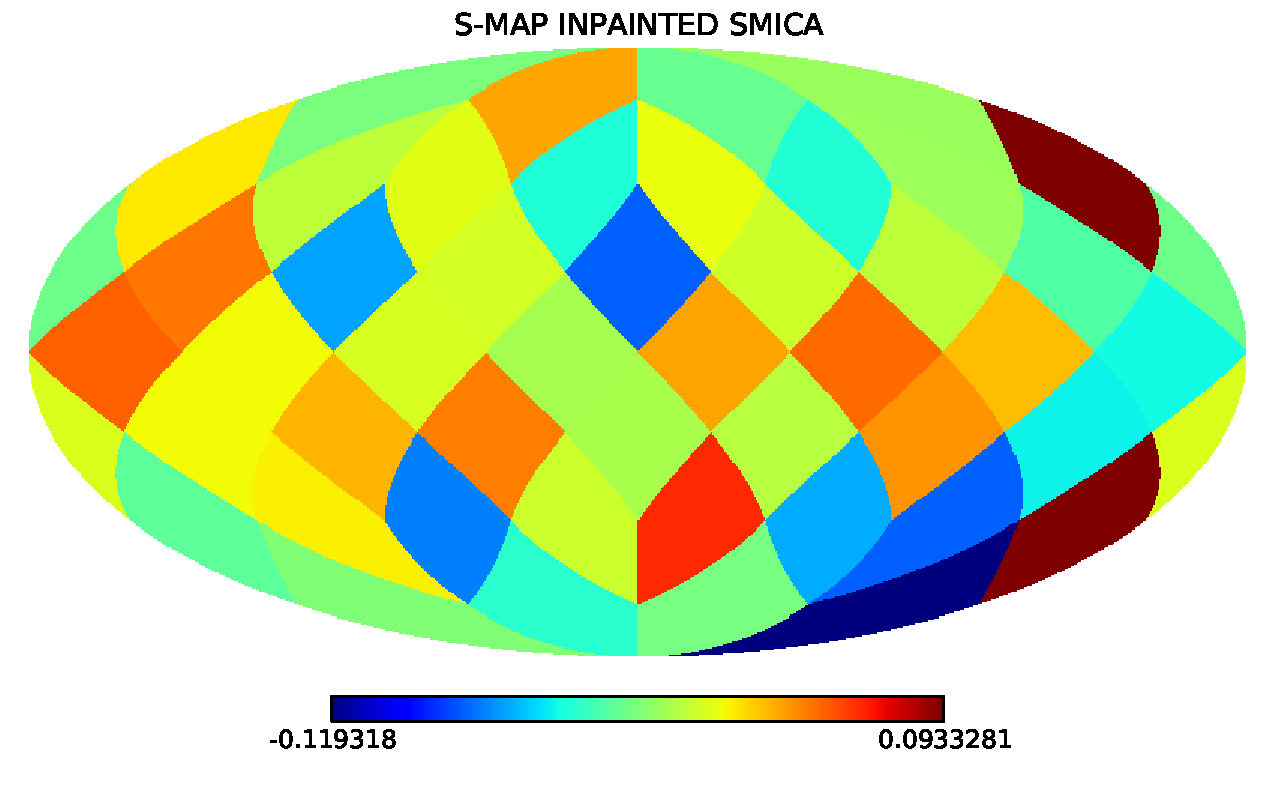
\includegraphics[width=\textwidth]{figures/chapter-vsk/smap-inpainted-smica.pdf}
\caption{$N'_{side = 2}$ S-map for the $N_{side} = 2048$ inpainted SMICA CMB estimate.}
\label{Fig:0b}
\end{figure}

\begin{figure}
\centering
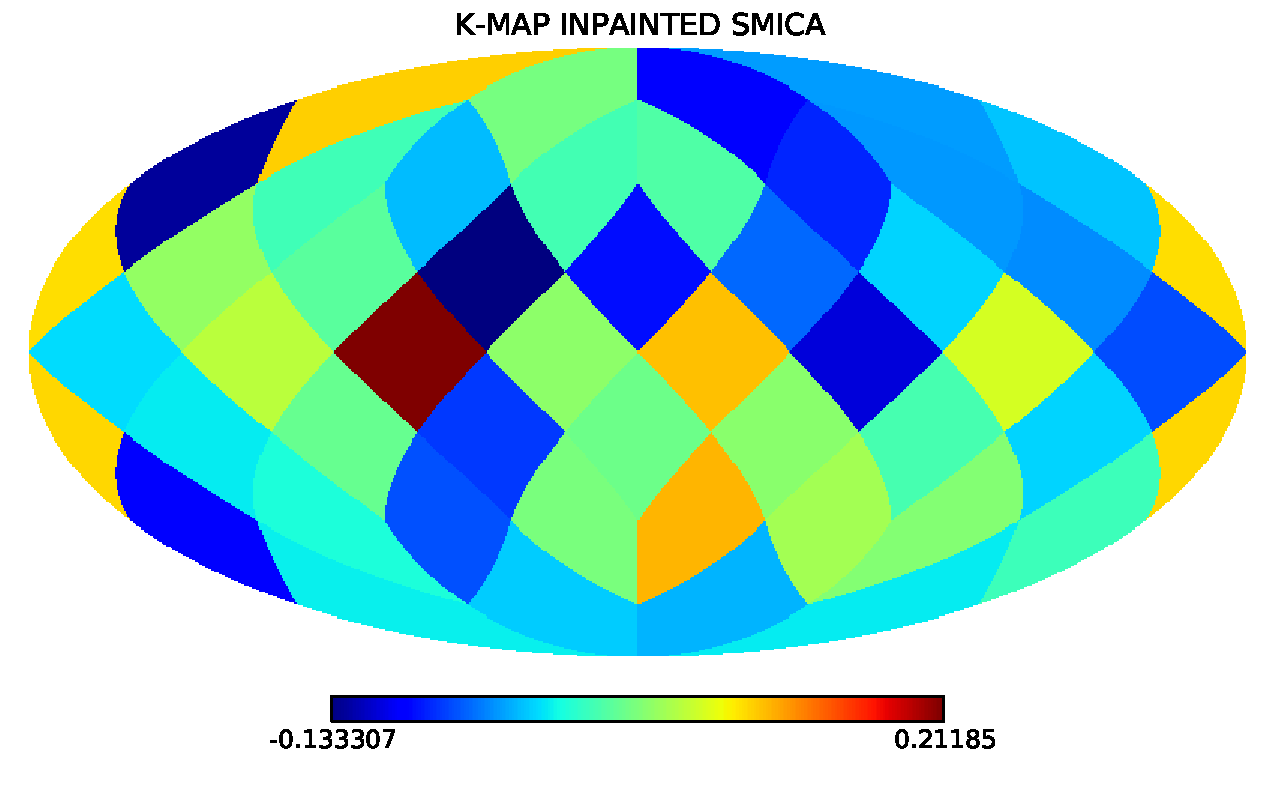
\includegraphics[width=\textwidth]{figures/chapter-vsk/kmap-inpainted-smica.pdf}
\caption{$N'_{side = 2}$ K-map for the $N_{side} = 2048$ inpainted SMICA CMB estimate.}
\label{Fig:0c}
\end{figure}


\begin{figure}
\centering
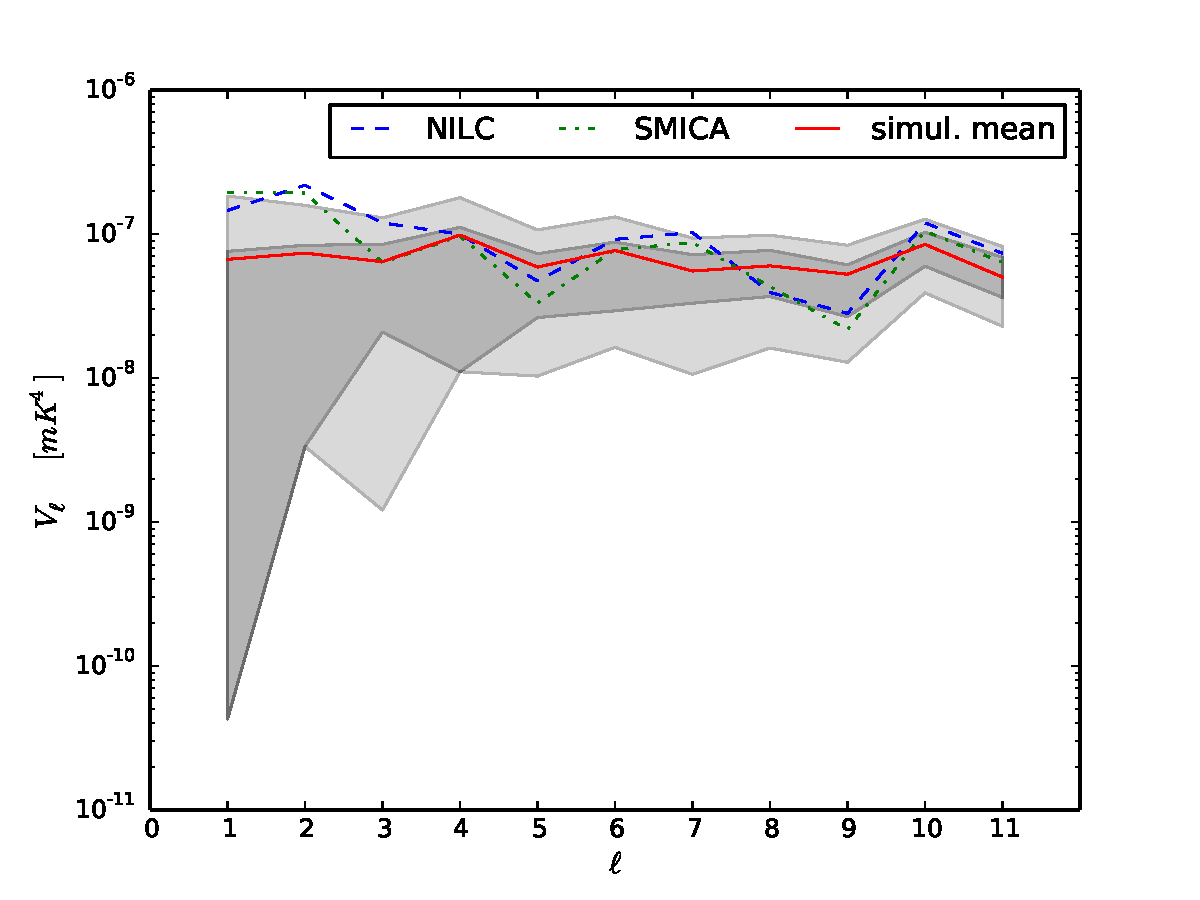
\includegraphics[width=\textwidth]{figures/chapter-vsk/Inp_Vl.pdf}
\caption{Angular power spectra for the $N'_{side} = 2$ V-map computed out of the full-sky $N_{side} = 2048$ inpainted CMB estimates. The red solid line indicates the mean for $1000$ Monte Carlo simulations and the shaded dark and light gray regions indicate the $68$ per cent and $95$ per cent confidence regions, respectively.}
\label{Fig:1}
\end{figure}

\begin{figure}
\centering
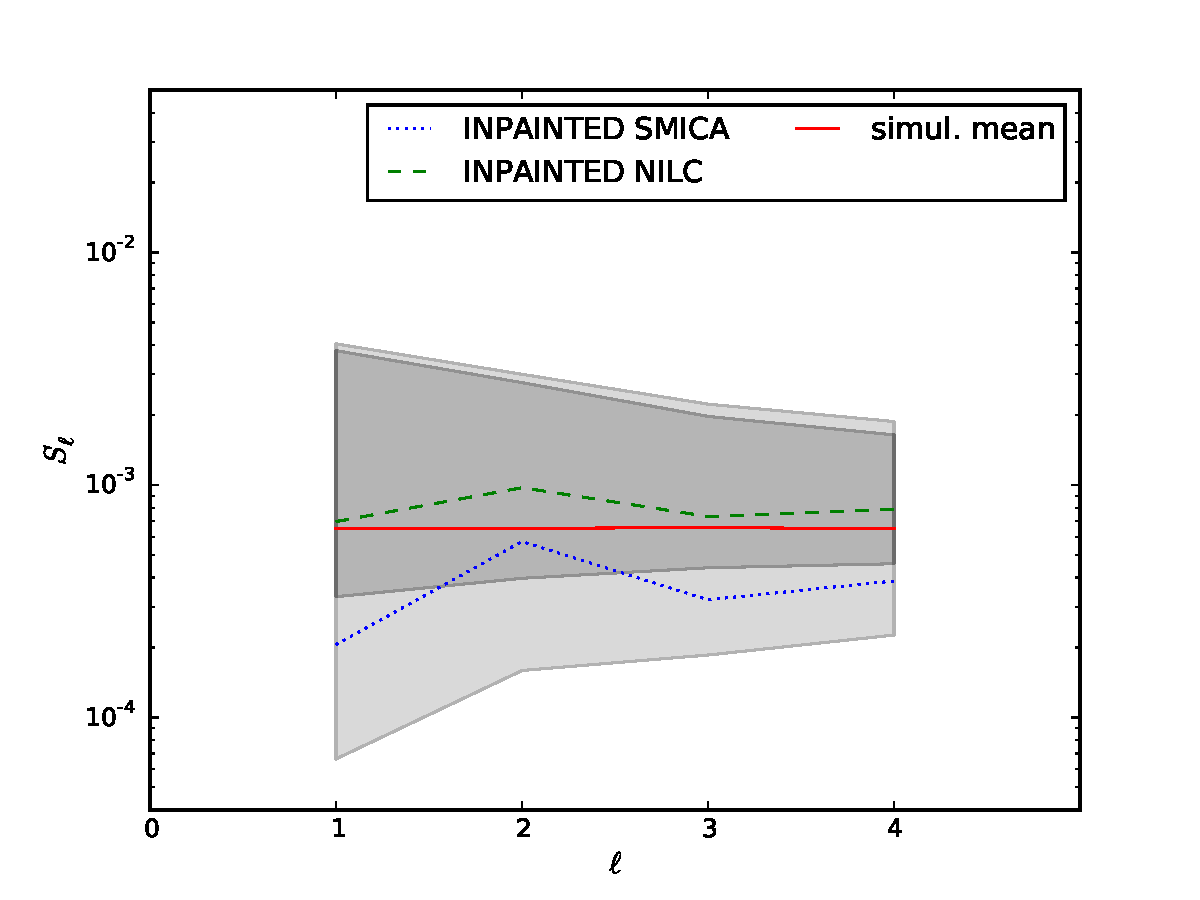
\includegraphics[width=\textwidth]{figures/chapter-vsk/Inp_Sl.pdf}
\caption{Angular power spectra for the $N'_{side} = 2$ S-map computed out of the full-sky $N_{side} = 2048$ inpainted CMB estimates. The red solid line indicates the mean for $1000$ Monte Carlo simulations and the shaded dark and light gray regions indicate the $68$ per cent and $95$ per cent confidence regions, respectively.}
\label{Fig:1a}
\end{figure}

\begin{figure}
\centering
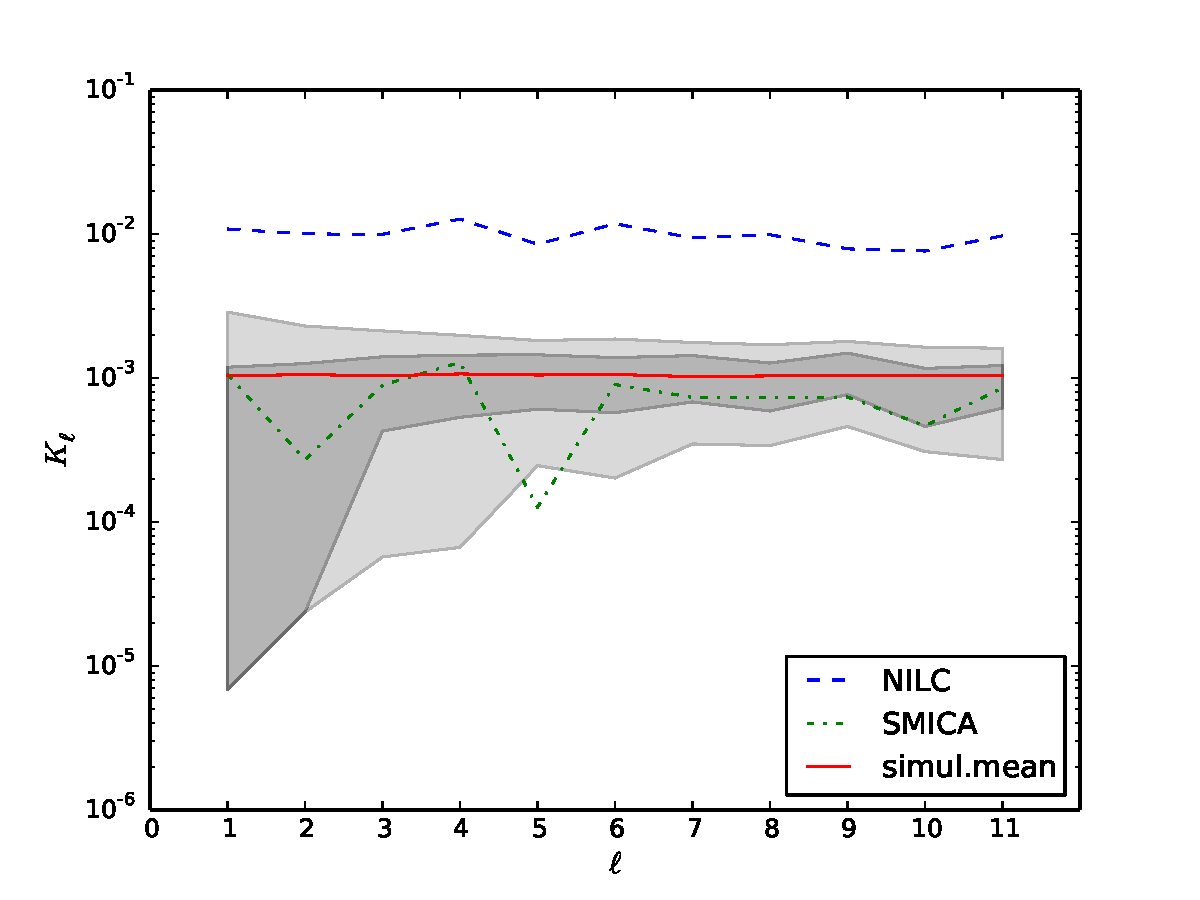
\includegraphics[width=\textwidth]{figures/chapter-vsk/Inp_Kl.pdf}
\caption{Angular power spectra for the $N'_{side} = 2$ K-map computed out of the full-sky $N_{side} = 2048$ inpainted CMB estimates. The red solid line indicates the mean for $1000$ Monte Carlo simulations and the shaded dark and light gray regions indicate the $68$ per cent and $95$ per cent confidence regions, respectively.}
\label{Fig:1b}
\end{figure}

\begin{figure}
\centering
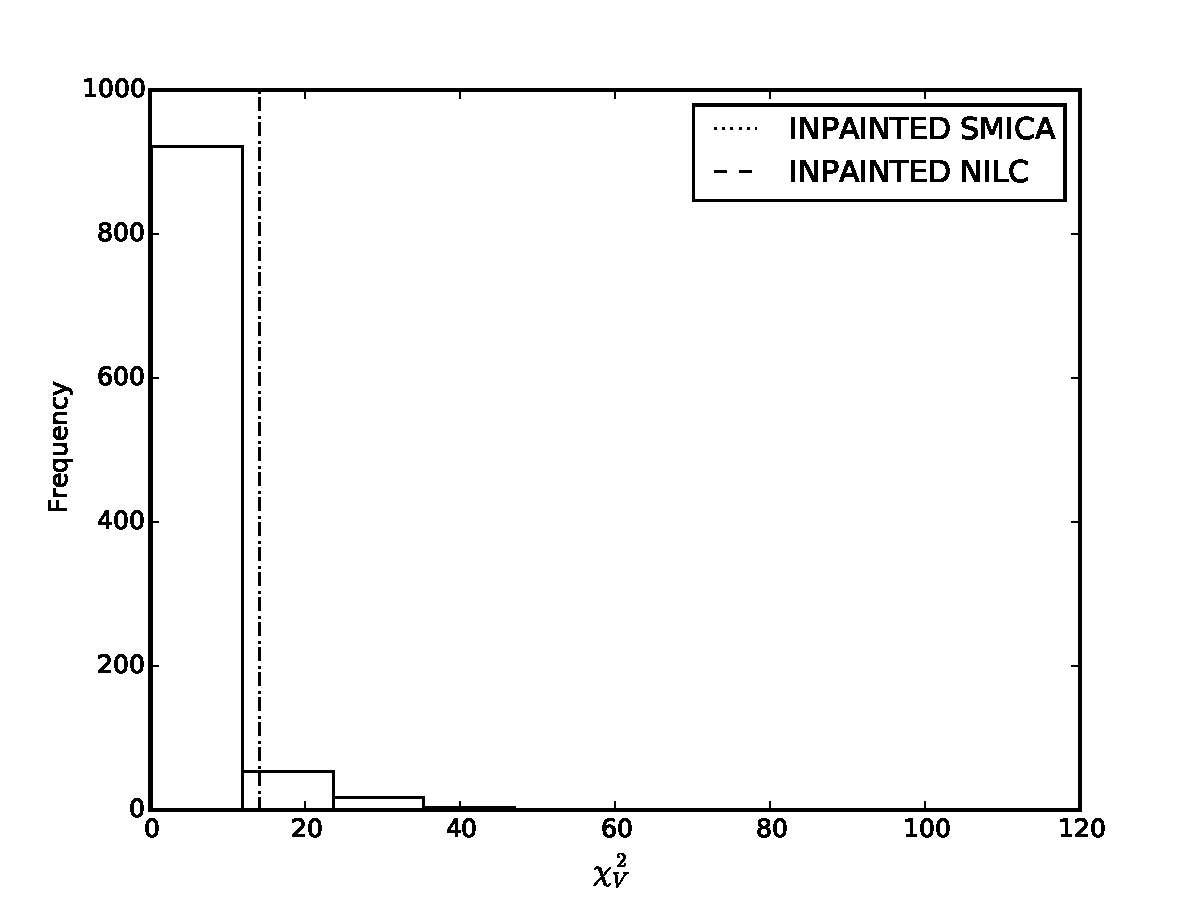
\includegraphics[width=\textwidth]{figures/chapter-vsk/vchi2.pdf}
\caption{N-pdf $\chi^ 2$ for the angular power spectra shown in Figure \ref{Fig:1}. The vertical lines show values for the corresponding CMB estimates.}
\label{Fig:2}
\end{figure}

\begin{figure}
\centering
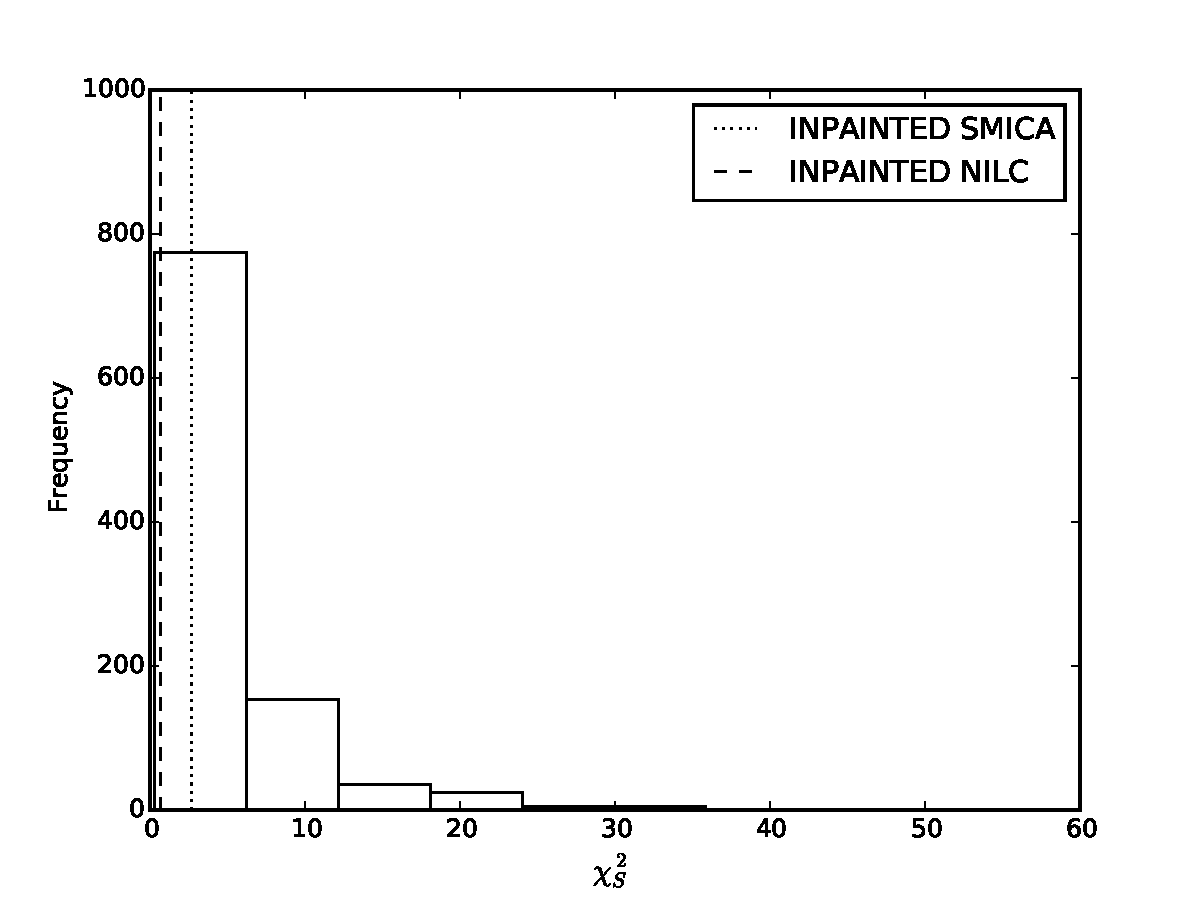
\includegraphics[width=\textwidth]{figures/chapter-vsk/schi2.pdf}
\caption{N-pdf $\chi^ 2$ for the angular power spectra shown in Figure \ref{Fig:1a}. The vertical lines show values for the corresponding CMB estimates.}
\label{Fig:2a}
\end{figure}

\begin{figure}
\centering
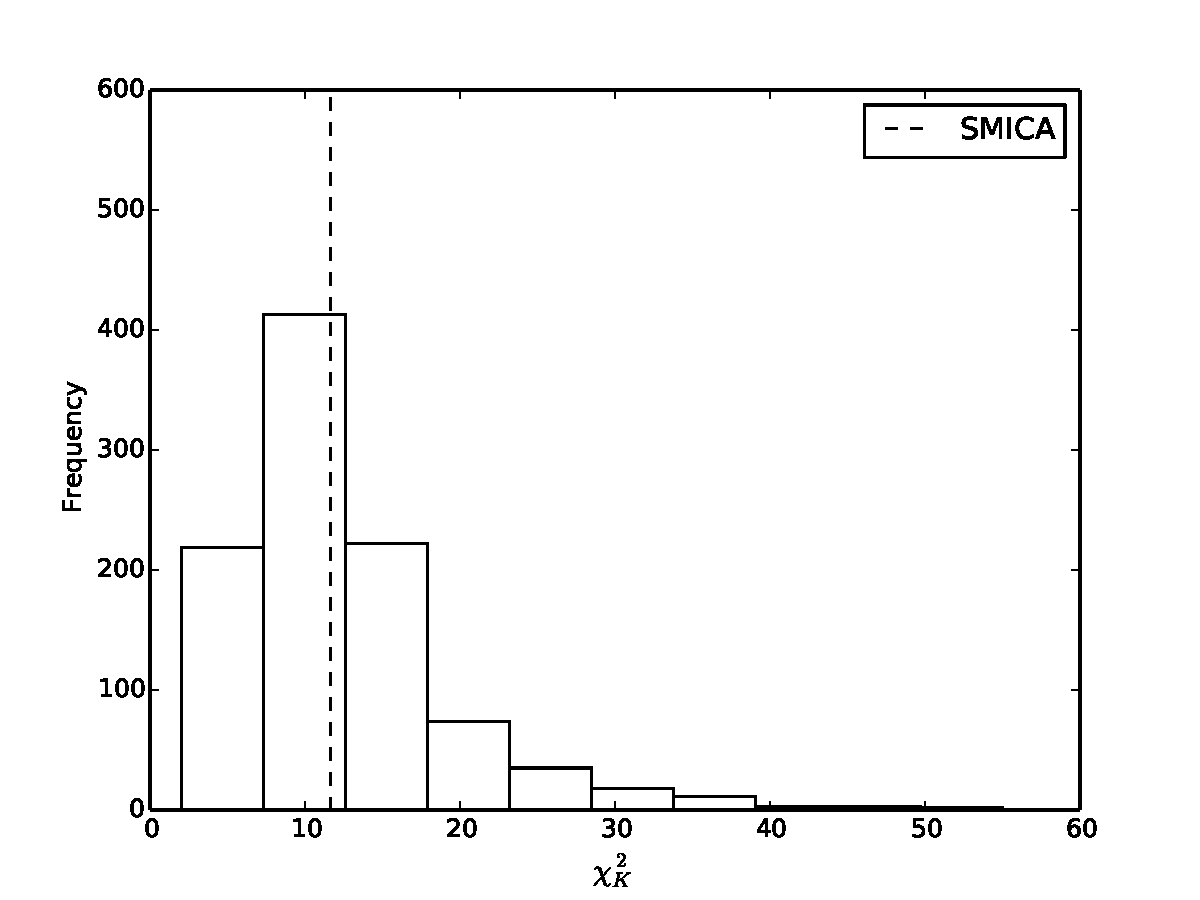
\includegraphics[width=\textwidth]{figures/chapter-vsk/kchi2.pdf}
\caption{N-pdf $\chi^ 2$ for the angular power spectra shown in Figure \ref{Fig:1b}. The vertical lines show values for the corresponding CMB estimates.}
\label{Fig:2b}
\end{figure}

\begin{table}
\centering
\caption{Lower-tail probability for the V, S, K estimators, for the $N_{side} = 2048$ inpainted \texttt{SMICA} and \texttt{NILC}.}
\label{table:1}
\begin{tabular}{@{}lcccc}
\hline 
  & & Probability & \\
\hline  
CMB estimate & V & S & K \\ 
\hline  
 & & $N'_{side}=2$ & \\
\texttt{SMICA} & $0.939$ & $0.388$ & $0.096$ \\ 
\texttt{NILC} & $0.939$ & $0.022$ & $1.0$  \\
%\texttt{SMICA} & $0.977$ & $0.355$ & $0.038$ \\ 
%\texttt{NILC} & $0.972$ & $0.781$ & $1.0$  \\
 & & $ N'_{side} = 4 $ & \\
\texttt{SMICA} & $ 0.969 $ & $ 0.727 $ & $ 0.521 $ \\
\texttt{NILC} & $ 0.943 $ & $ 0.761 $ & $ 1.0 $ \\ 
%\texttt{SMICA} & $0.998$ & $0.718$ & $0.585$ \\
%\texttt{NILC} & $0.985$ & $0.988$ & $1.0$ \\
 & & $N'_{side} = 8$ & \\
\texttt{SMICA} & $ $ & $ $ & $ $ \\
\texttt{NILC} & $ $ & $ $ & $ $ \\
% \texttt{SMICA} & $1.0$ & $0.374$ & $0.745$ \\
% \texttt{NILC} & $0.995$ & $0.385$ & $1.0$ \\
% & & $N'_{side} = 16$ & \\
%\texttt{SMICA} & $ $ & $ $ & $ $ \\
%\texttt{NILC} & $ $ & $ $ & $ $ \\
% \texttt{SMICA} & $1.0$ & $0.241$ & $0.786$ \\
% \texttt{NILC} & $1.0$ & $0.093$ & $1.0$ \\
\hline
\end{tabular} 
\end{table}

According to the previous analysis the inpainting technique applied to \texttt{NILC} might induce deviations of the null hypothesis. We now apply the VSK method to the almost full-sky $N_{side}=2048$ CMB estimates; we examine the four component separation methods mentioned above and use the U73 mask. In Figures \ref{Fig:3}--\ref{Fig:3b} we illustrate, as an example, the V-map, S-map, and the K-map for the \texttt{SMICA} estimate. In Figures \ref{Fig:4}--\ref{Fig:4b} we plot the corresponding angular power spectra $V_{\ell},\, S_{\ell},\, $ and $K_{\ell}$ computed for the four component separation CMB estimates. Since all the four CMB estimates are consistent with the null hypothesis, we conclude the inpainting technique applied to the \texttt{NILC} CMB map causes the discrepancy we noted before (see Figure \ref{Fig:1b}). %Nevertheless, note that due to the masked regions in the V-maps, S-maps, and K-maps the angular power spectra of the simulations are not any longer scale independent, the effect being much more visible in the case of $V_{\ell}$ because of the much more different value associated with the masked pixels. 

A modification in the VSK method to include only unmasked regions in the computation of the angular power spectrum would be necessary. This would allow to know the true shape of the angular power spectra and avoid spurious features possibly induced by the masked region. Nevertheless, since in this work we want to test whether or not the \textit{Planck} data are consistent with the null hypothesis, we will not include  this modification in the present chapter. Such a modification would require to adapt the VSK method as explained in \cite{Gorski:1994ye} and \cite{Hivon:2001jp}. The code \textsc{PolSpice} can analyse functions on the cut-sky, correcting the effects of the masks. An adaptation of the VSK method using \textsc{PolSpice} is under development. 

%Comparing the results of the full-sky inpainted CMB maps with those of the almost full-sky CMB maps, we can see that there is no departure from the null hypothesis in the NILC CMB estimate when the inpainted regions are disregarded. Thus, the discrepancy observed in the full-sky map for the K estimator seems to be caused by the inpainted regions in the inpainted \texttt{NILC}. 
None of the four component separation methods exhibits a dipole in the V-maps outside the $95$ per cent confidence region for $N'_{side}=2$. %We are testing whether this result depends on the parameter $N'_{side}$. % This might be due to the fact that by construction the method VSK, as we have applied it here, disregards patches (patches set to zero) with less than $80$ per cent of unmasked pixels and therefore it is not guaranteed that the sky fraction (fraction of the sky having patches with non zero value) be the same for each $N'_{side}$. 
Since all the four component separation methods give pretty similar results and to avoid circumlocution, in Table \ref{table:2} we present the lower-tail probabilities only for the \texttt{SMICA} CMB estimate masked with the U73 mask. We are examining the dependence of our results on the parameters $N_{side}$ and $N'_{side}$. Thus far, we do not see significant deviation of the null hypothesis for almost all the possible combinations of parameters considered.%, with the exception of the V estimator for $N_{side}=2048$ and $N'_{side}=8,\,16$ where there is a discrepancy with the simulations.
 

\begin{figure}
\centering
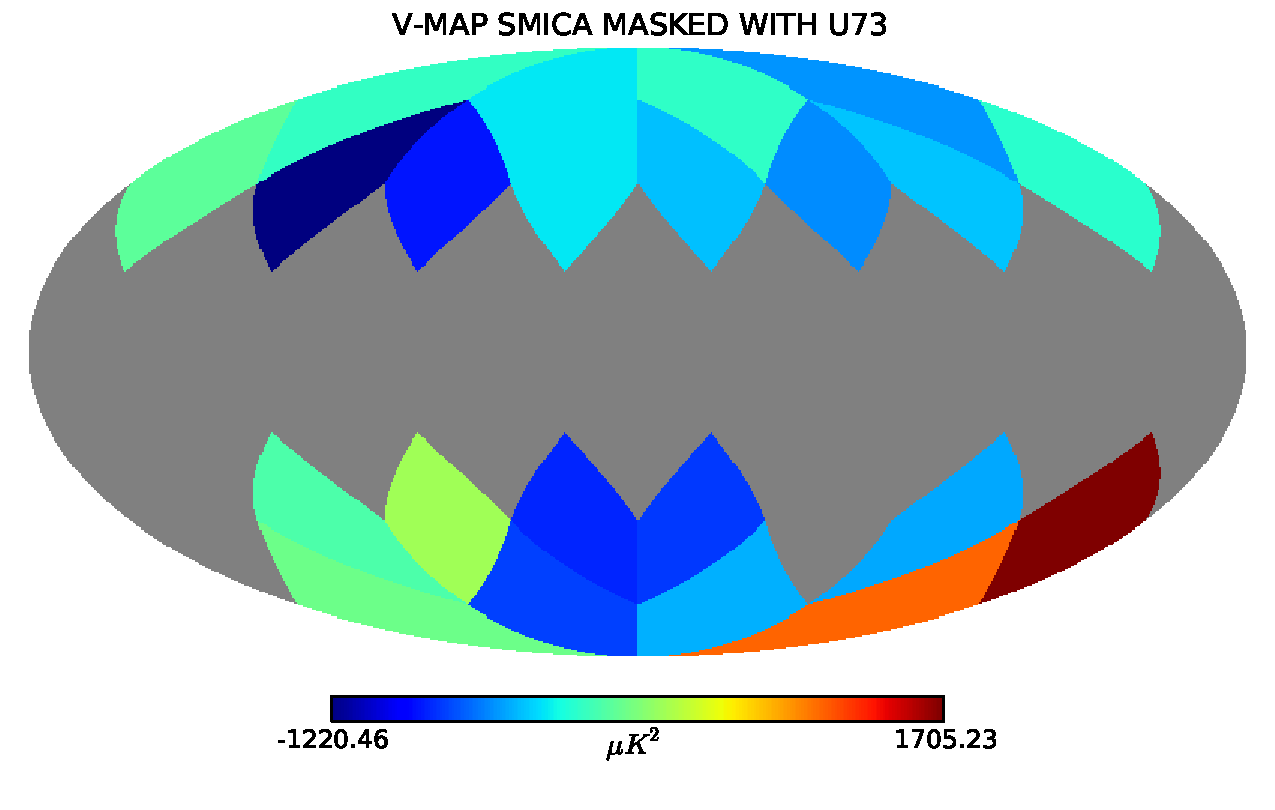
\includegraphics[width=\textwidth]{figures/chapter-vsk/vmap-u73-smica.pdf}
\caption{$N'_{side = 2}$ V-map for the $N_{side} = 2048$ SMICA CMB estimate masked with the U73 mask.}
\label{Fig:3}
\end{figure}

\begin{figure}
\centering
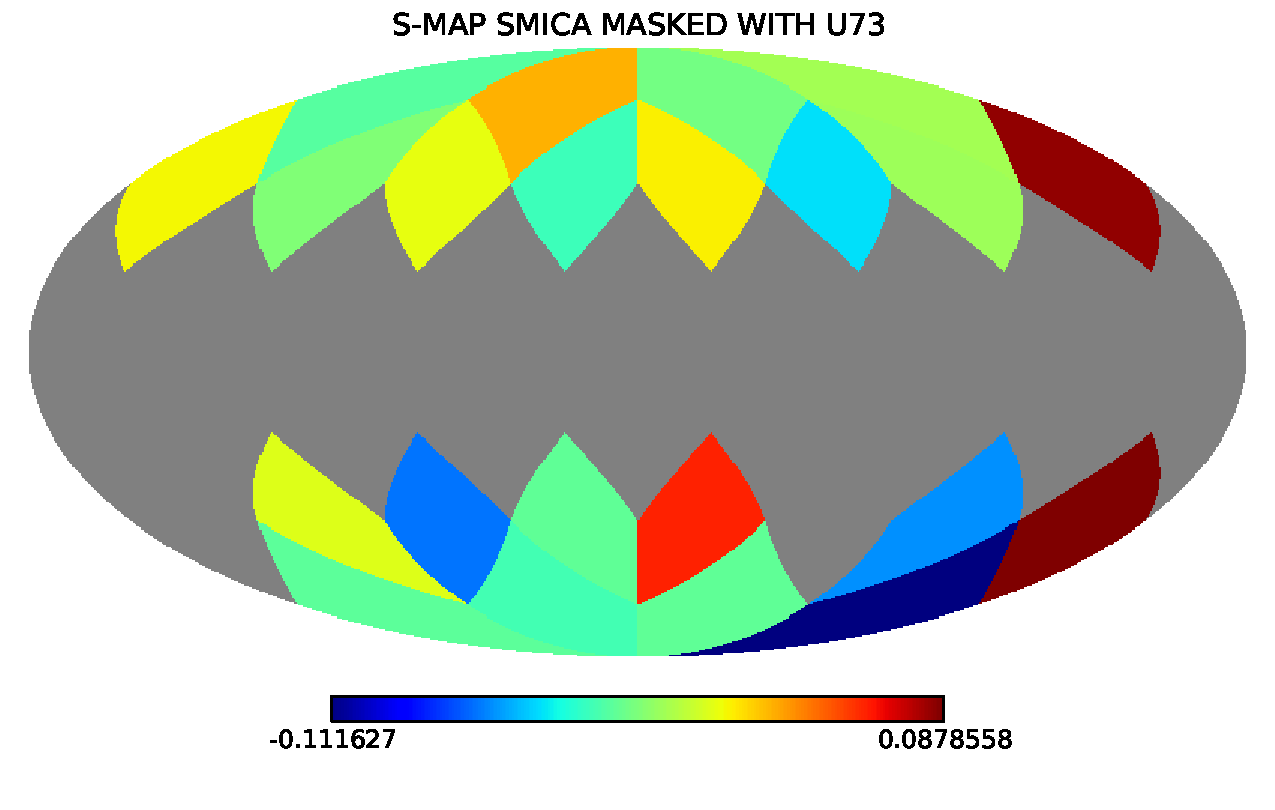
\includegraphics[width=\textwidth]{figures/chapter-vsk/smap-u73-smica.pdf}
\caption{$N'_{side = 2}$ S-map for the $N_{side} = 2048$ SMICA CMB estimate masked with the U73 mask.}
\label{Fig:3a}
\end{figure}

\begin{figure}
\centering
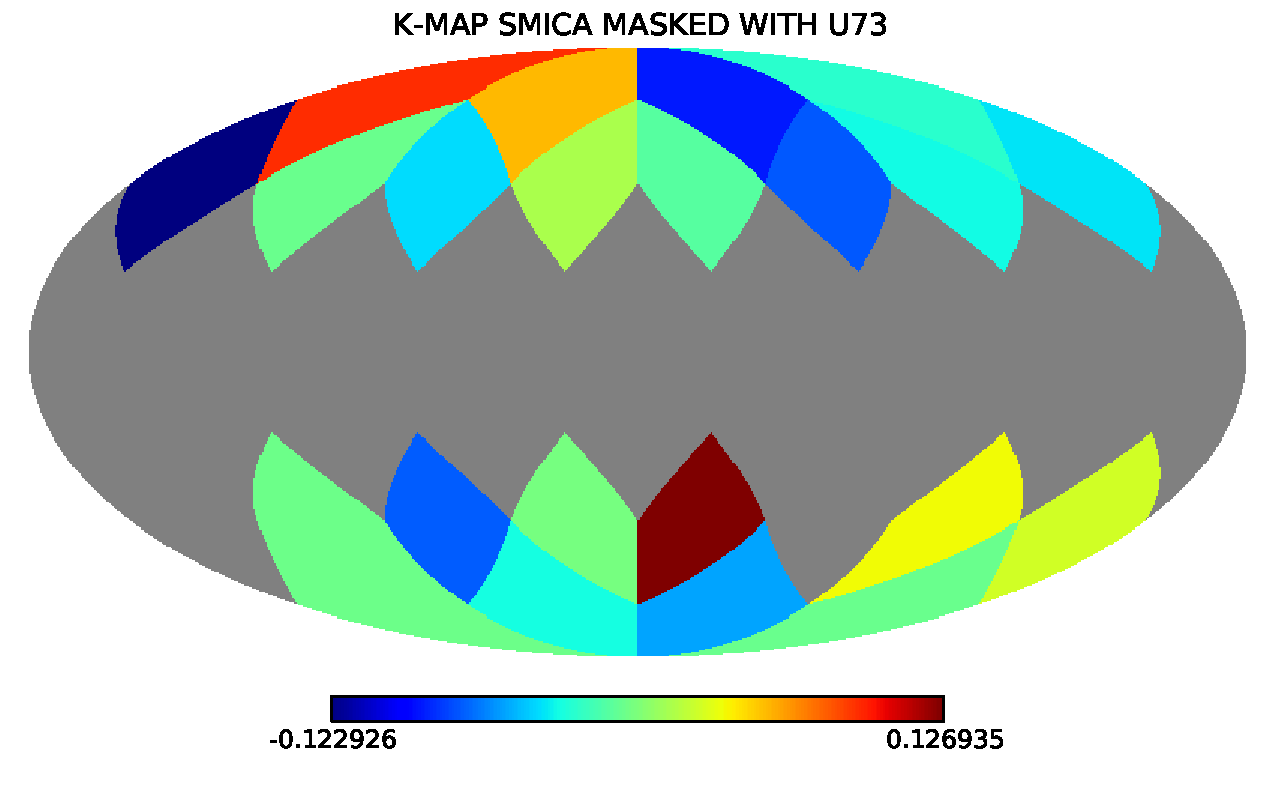
\includegraphics[width=\textwidth]{figures/chapter-vsk/kmap-u73-smica.pdf}
\caption{$N'_{side = 2}$  K-map for the $N_{side} = 2048$ SMICA CMB estimate masked with the U73 mask.}
\label{Fig:3b}
\end{figure}

\begin{figure}
\centering
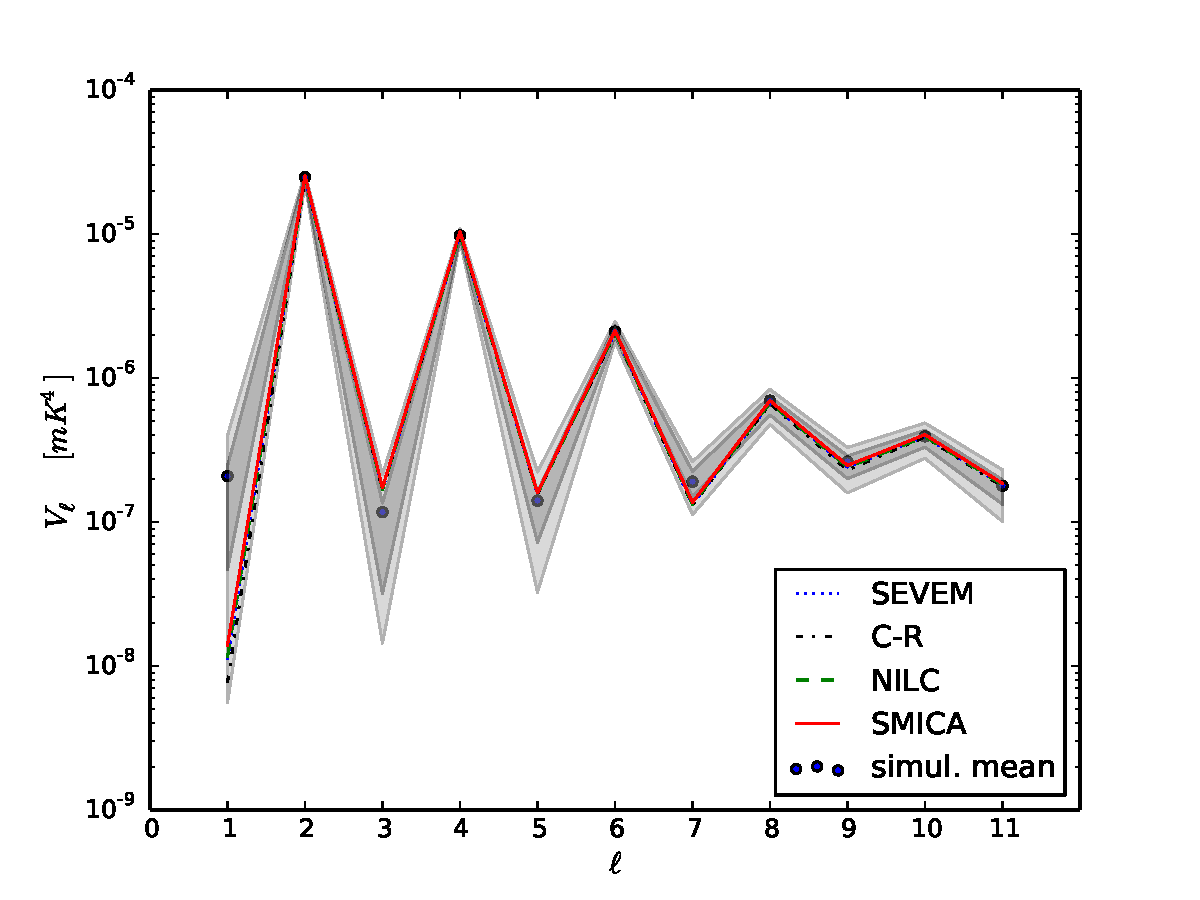
\includegraphics[width=\textwidth]{figures/chapter-vsk/Vl_u73.pdf}
\caption{Angular power spectra of the $N'_{side} = 2$ V-map for the four $N_{side} = 2048$ CMB estimates. The magenta line indicates the mean angular power spectrum for $1000$ Monte Carlo simulations and the shaded dark and light gray regions indicate the $68$ per cent and $95$ per cent confidence regions, respectively.}
\label{Fig:4}
\end{figure}

\begin{figure}
\centering
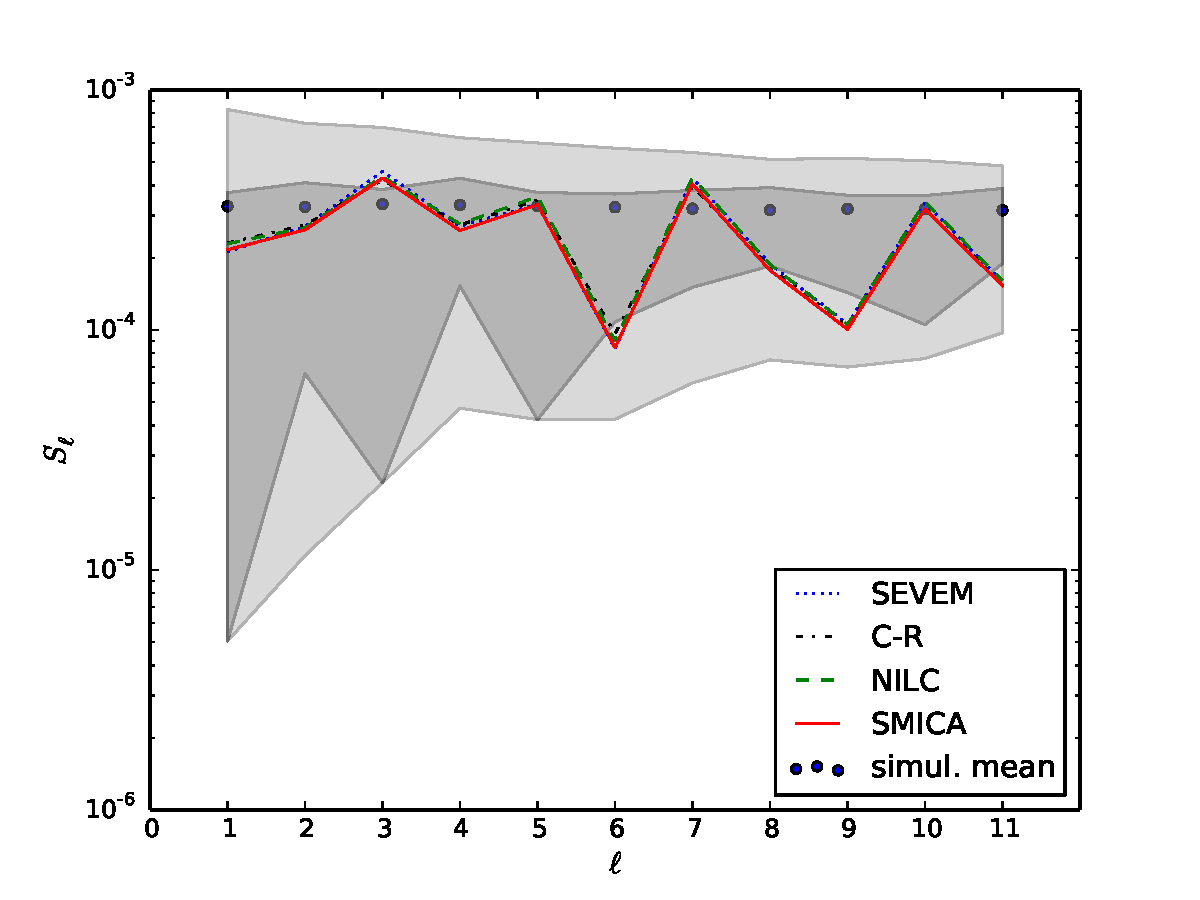
\includegraphics[width=\textwidth]{figures/chapter-vsk/Sl_u73.pdf}
\caption{Angular power spectra of the $N'_{side} = 2$ S-map for the four $N_{side} = 2048$ CMB estimates. The magenta line indicates the mean angular power spectrum for $1000$ Monte Carlo simulations and the shaded dark and light gray regions indicate the $68$ per cent and $95$ per cent confidence regions, respectively.}
\label{Fig:4a}
\end{figure}

\begin{figure}
\centering
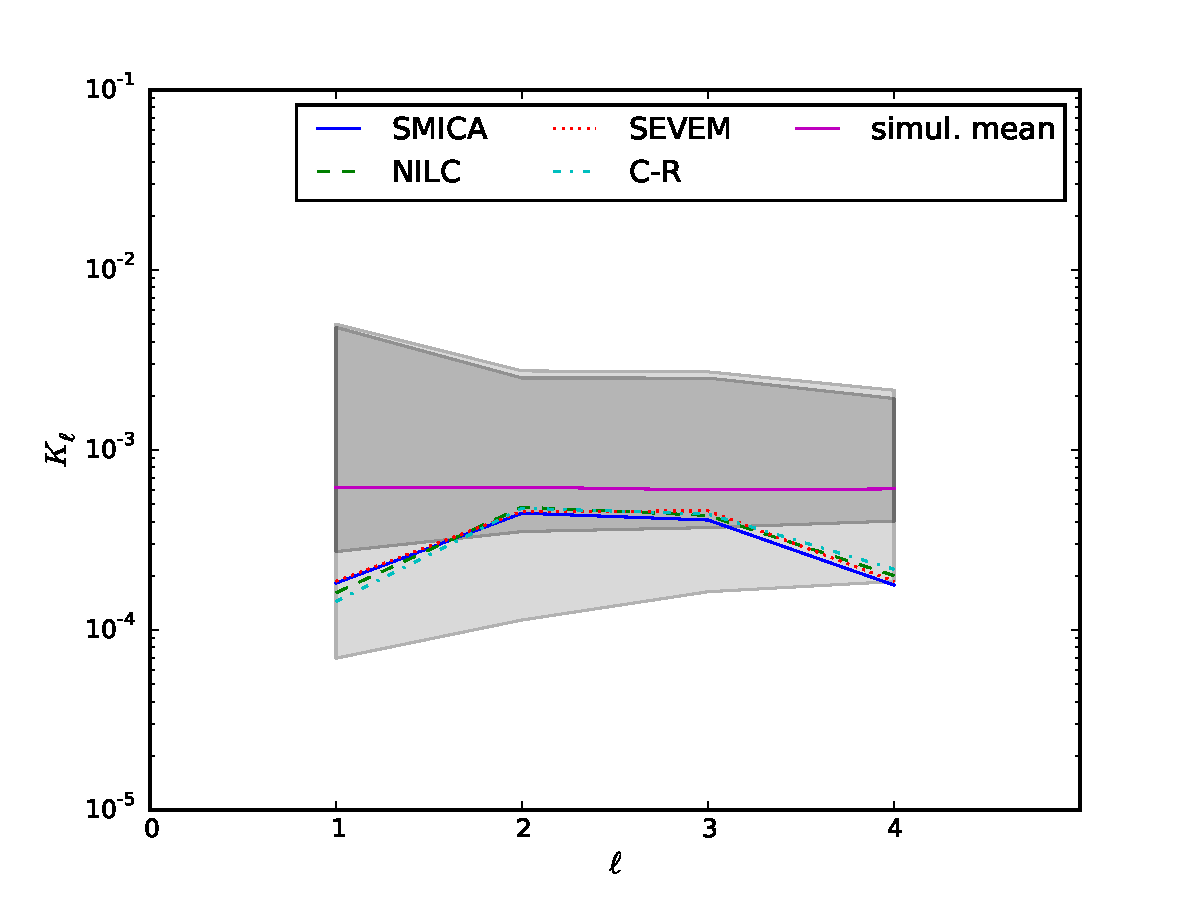
\includegraphics[width=\textwidth]{figures/chapter-vsk/Kl_u73.pdf}
\caption{Angular power spectra of the $N'_{side} = 2$ K-map for the four $N_{side} = 2048$ CMB estimates. The magenta line indicates the mean angular power spectrum for $1000$ Monte Carlo simulations and the shaded dark and light gray regions indicate the $68$ per cent and $95$ per cent confidence regions, respectively.}
\label{Fig:4b}
\end{figure}

Since discrepancies might arise due to unresolved foregrounds, we are also investigating how our results depend on the masked region. The results for both the confidence mask and the mask of inpainted regions for \texttt{SMICA} are shown in Table \ref{table:3}. In order to facilitate the comparison, some of the results for the mask U73 are repeated. %The sky coverage of the considered masks does not seem to affect the results considerably in any of the estimators. 

\begin{table}
\centering
\caption{Lower-tail probability for the V, S, K estimators using different $N'_{side}$, for different resolutions $N_{side}$ of the  \texttt{SMICA} CMB estimate using the U73 mask.}
\label{table:2}
\begin{tabular}{@{}lcccc}
\hline 
  & & Probability & \\
\hline  
$N'_{side}$ & V & S & K \\ 
\hline  
 & & $N_{side}=2048$ & \\
$2$ & $0.004 $ & $ 0.024$ & $0.367 $ \\ 
%$2$ & $0.929 $ & $ 0.152$ & $0.513 $ \\ 
%$4$ & $ 0.754$ & $0.656 $ & $0.292 $  \\
%$8$ & $ 1.0$ & $ 0.094 $ & $ 0.412 $  \\
%$16$ & $ 1.0 $ & $ 0.391 $ & $ 0.439 $  \\
%$2$ & $0.929 $ & $ 0.152$ & $0.513 $ \\ 
$4$ & $ $ & $ $ & $ $  \\
$8$ & $ $ & $  $ & $  $  \\
%$16$ & $  $ & $  $ & $  $  \\
 & & $ N_{side} = 1024 $ & \\
$2$ & $ 0.556 $ & $ 0.022 $ & $ 0.281 $ \\ 
%$2$ & $ 0.869 $ & $ 0.151 $ & $ 0.523 $ \\ 
$4$ & $ 0.873 $ & $ 0.446 $ & $ 0.229 $  \\
$8$ & $  $ & $  $ & $  $  \\
$16$ & $ 0.442 $ & $ 0.084 $ & $ 0.153 $  \\
%$4$ & $ 0.394 $ & $ 0.653 $ & $ 0.253 $  \\
%$8$ & $ 0.835 $ & $ 0.145 $ & $ 0.457 $  \\
%$16$ & $ 0.928 $ & $ 0.226 $ & $ 0.265 $  \\
 & & $N_{side} = 512$ & \\
$2$ & $0.711 $ & $ 0.027 $ & $ 0.229 $ \\ 
%$2$ & $0.273 $ & $ 0.174 $ & $ 0.626 $ \\ 
$4$ & $ 0.898 $ & $ 0.485 $ & $ 0.240 $  \\
%$4$ & $ 0.532 $ & $ 0.651 $ & $ 0.195 $  \\
$8$ & $ 0.794 $ & $ 0.103 $ & $ 0.140 $  \\
$16$ & $ 0.311 $ & $ 0.200 $ & $ 0.146 $  \\
%$8$ & $ 0.5 $ & $ 0.167 $ & $ 0.559 $  \\
%$16$ & $ 0.492 $ & $ 0.231 $ & $ 0.331 $  \\
 & & $N_{side} = 256$ & \\
$2$ & $ 0.040 $ & $ 0.123 $ & $ 0.225 $ \\ 
%$2$ & $ 0.276 $ & $ 0.235 $ & $ 0.647 $ \\ 
$4$ & $ 0.996 $ & $ 0.480 $ & $ 0.404 $  \\
%$4$ & $ 0.393 $ & $ 0.571 $ & $ 0.232 $  \\
%$8$ & $ 0.192 $ & $ 0.216 $ & $ 0.518 $  \\
%$16$ & $ 0.589$ & $ 0.176 $ & $ 0.409 $  \\
$8$ & $ 1.0 $ & $ 0.235 $ & $ 0.104 $  \\
$16$ & $ 1.0$ & $ 0.584 $ & $ 0.459 $  \\
\hline
\end{tabular} 
\end{table}

\begin{table}
\centering
\caption{Lower-tail probability for the V, S, K estimators at $N'_{side}=2$, for the \texttt{SMICA} CMB estimate using different masks.}
\label{table:3}
\begin{tabular}{@{}lcccc}
\hline 
  & & Probability & \\
\hline  
$N'_{side}$ & V & S & K \\ 
\hline  
 & & U73 ($f_{sky} = 73\%$) & \\
$2$ & $ 0.004 $ & $ 0.024 $ & $ 0.367 $ \\ 
%$2$ & $ 0.929 $ & $ 0.152 $ & $ 0.513 $ \\ 
%$4$ & $ 0.754 $ & $ 0.656 $ & $ 0.292 $  \\
$4$ & $ 0.893 $ & $ 0.407 $ & $ 0.340 $  \\
$8$ & $  $ & $  $ & $  $  \\
%$16$ & $  $ & $  $ & $  $  \\
 & & VALMASK ($f_{sky} = 89\%$) & \\
$2$ & $ 0.004 $ & $ 0.022 $ & $ 0.357 $ \\ 
$4$ & $ 0.895 $ & $ 0.371 $ & $ 0.343 $  \\
$8$ & $  $ & $  $ & $  $  \\
%$16$ & $  $ & $  $ & $  $  \\
%$2$ & $ 0.983 $ & $ 0.388 $ & $ 0.423 $ \\ 
%$4$ & $ 0.741 $ & $ 0.754 $ & $ 0.319 $  \\
 & & INP$\_$MASK ($f_{sky} = 97\%$) & \\
$2$ & $ 0.003 $ & $ 0.016 $ & $ 0.382 $ \\ 
$4$ & $ 0.897 $ & $ 0.367$ & $ 0.374 $  \\
$8$ & $  $ & $  $ & $  $  \\
%$16$ & $  $ & $  $ & $  $  \\
%$2$ & $ 0.976 $ & $ 0.37 $ & $ 0.163 $ \\ 
%$4$ & $ 0.996 $ & $ 0.738 $ & $ 0.528 $  \\
\hline
\end{tabular} 
\end{table}


\section{Conclusions}
\label{s:summary}

In this chapter we carried out a non-parametric analysis, the VSK method, to test for possible departures from the cosmological principle in the CMB anisotropies measured by the \textit{Planck} satellite. We used the available full-sky maps (inpainted \texttt{SMICA} and \texttt{NILC}) and the four almost full-sky CMB estimates released in 2013 by the \textit{Planck} collaboration (\texttt{SMICA, NILC, Commander-Ruler,} and \texttt{SEVEM}). We investigated possible anomalous angular variations of the variance, skewness, and kurtosis in the CMB anisotropies and determined the statistical significance of our results by using a set of Gaussian, isotropic simulations of the CMB sky seeded by the \textit{Planck} best-fit angular power spectrum.    

The VSK method applied to inpainted \textit{Planck} maps brings about the following features. The V estimator indicates no departure ($95$ per cent confidence region) of the null hypothesis at the level of the dipole and the quadrupole. Thus far, these results are robust against both component separation and the parameter $ N'_{side} $ of the VSK method. The S estimator is fully consistent with the null hypothesis in both CMB estimates. This is not the case for the K estimator, where only inpainted \texttt{SMICA} turns out to be consistent with the simulations. According to the K estimator, the inpainting method applied to \texttt{NILC } induces kurtosis on all scales allowed by a given $ N'_{side} $. It remains to be seen  whether or not this discrepancy with the null hypothesis becomes  less significant when higher $ N'_{side} $ is employed.  

We studied several aspects of the VSK method applied to the almost full-sky \textit{Planck} maps. In particular, we considered the VSK method applied to the four component separation CMB estimates by using different resolutions of the data ($ N_{side} $), masks, and $ N'_{side} $. Thus far, all the four component separation methods are fully consistent with the hypothesis of a universe statistically isotropic and Gaussian regardless of these parameters of the VSK method. It remains to be seen, however, whether the VSK method using a larger sky fraction of the sky would bring about anomalies such as north-south asymmetry or quadrupole alignment.    

When applying the VSK method to masked CMB maps one must be careful. Since the method computes the full-sky angular power spectrum of V-map, S-map, and K-map, the masked region of those maps might include spurious correlations. %angular variations if the value of the unmasked pixels is very different from the masked ones.  
A modified VSK method should take into account only unmasked pixels of the V-map, S-map, and K-map and use orthogonal functions on the cut sphere in order to avoid this caveat. Since both the simulations and the data are affected in the same way by this limitation of the method, such a modification might not alter our results (consistency with the null hypothesis), but produce the true shape of the angular power spectra.  

Finally, we notice that %although our results are compatible with most of the analysis done by the \textit{Planck} team, a direct comparison is not possible. First, by construction, the VSK method may not use the same fraction of the sky as analysed by some of the statistical methods used by the \textit{Planck} team. 
the results presented in this chapter are just preliminary and the project is ongoing. The 2015 \textit{Planck} data is now available and includes a sophisticated set of Gaussian, isotropic simulations  (the FFP8 simulations). These simulations are maps of the CMB for the different frequencies in the \textit{Planck} satellite. Since we have shown that the four component separation methods are in agreement with each other when analysed with the VSK method, the use of the FFP8 simulations in this project would require the implementation of at least one the component separation methods. We plan to do this for the \texttt{SEVEM} component separation. Another additional point worthy of further investigation would be the dependence of the results with CMB frequency. These two additional points -- use of FFP8 simulations and frequency dependence -- would make possible a direct comparison with the results found by the \textit{Planck} team. 
